% -----------------------------------------------
% Modelo UFT para Trabalhos Acadêmicos
% Adaptado e mantido por Wenes (Libertário)
% Baseado no projeto abnTeX2, porém modificado para atender às diretrizes
% visuais e estruturais da Universidade Federal do Tocantins (UFT).
% Esta versão não é oficial e não substitui os modelos originais do abnTeX2.
% -----------------------------------------------
\documentclass[
	12pt,				% Tamanho da fonte
    oneside,            % Garante margens iguais (não alternadas)
	a4paper,			% tamanho do papel. 
	english,			% idioma adicional para hifenização
	brazilian,		    % o último idioma é o principal do documento
	]{abntex2}
% -----------------------------------------------


% -----------------------------------------------
% -------------Pacotes fundamentais-------------- 
% -----------------------------------------------
\usepackage{lmodern}			% Usa a fonte Latin Modern		
\usepackage[T1]{fontenc}		% Seleção de códigos de fonte.
\usepackage[utf8]{inputenc}		% Codificação do documento (conversão automática dos acentos)
\usepackage{indentfirst}		% Indenta o primeiro parágrafo de cada seção.
\usepackage{color}				% Controle das cores
\usepackage{graphicx}			% Inclusão de gráficos
\usepackage{microtype} 			% para melhorias de justificação
% -----------------------------------------------


% -----------------------------------------------
\usepackage{lipsum}	% para geração de texto------
% -----------------------------------------------


% -----------------------------------------------
% -------------Pacotes de citações---------------
% -----------------------------------------------
\usepackage[backend=biber,style=abnt,language=brazil]{biblatex}
\addbibresource{Referencias.bib}
\usepackage{csquotes}             % Recomendado pelo biblatex 
\usepackage{etoolbox}             % Auxilia na justificação da bibliografia
\AtBeginBibliography{\justifying} % Ativa a justificação da bibliografia
\usepackage{ragged2e}
% -----------------------------------------------


% -----------------------------------------------
% --------VISUALIZAÇÃO E ESTABILIDADE------------
% -----------------------------------------------
\usepackage{tikz}         % Gerar imagem de exemplo
\usepackage{pgfplots}     % Funções matemática
\pgfplotsset{compat=1.18} % Garante compatibilidade
\usepackage{subcaption}   % Permite criar subfaturas
\usepackage{float}        % Adiciona a opção de posicionamento
\usepackage{amssymb}      % Necessário para símbolos matemáticos
\usepackage{amsmath}      % Necessário para comandos como \text{}


% -----------------------------------------------
% Informações de dados para CAPA e FOLHA DE ROSTO
% -----------------------------------------------
\titulo{Modelo UFT para\\ Trabalha de Conclusão de Curso\\ em \abnTeX}
\autor{Editado por Wenes Aquino}
\local{Palmas}
\data{2025, v-1.0}
\orientador{Editado por Wenes Aquino}
\coorientador{Editado por Wenes Aquino}

\instituicao{%
  Universidade Federal do Tocantins - UFT\\
  Campus Universitário de Palmas\\
  Curso de Licenciatura em Computação}
  
\tipotrabalho{Trabalho de Conclusão de Curso}

\preambulo{Trabalho de conclusão de curso apresentado como parte dos requisitos para avaliação na Universidade Federal do Tocantins (UFT). Este modelo foi adaptado e personalizado com ajustes visuais, estruturais e técnicos, servindo também para testar o espaço disponível e a formatação utilizada na contracapa deste documento.}
% -----------------------------------------------


% -----------------------------------------------
\makeatletter
\hypersetup{
    colorlinks=false,   % Desativa links coloridos
    pdfborder={0 0 0},  % Remove o retângulo ao redor dos links
}
\makeatother
% -----------------------------------------------


% -----------------------------------------------
% Posiciona figuras e tabelas no topo da página quando adicionadas sozinhas
% em um página em branco. Ver https://github.com/abntex/abntex2/issues/170
\makeatletter
\setlength{\@fptop}{5pt} % Set distance from top of page to first float
\makeatother
% -----------------------------------------------


% -----------------------------------------------
% ----Espaçamentos entre linhas e parágrafos----- 
% -----------------------------------------------
\setlength{\parindent}{1.3cm} % O tamanho do parágrafo é dado por:
\setlength{\parskip}{0.2cm}   % Espaçamento entre parágrafo
% -----------------------------------------------



% -----------------------------------------------
% ---------------Compila o Índice----------------
% -----------------------------------------------
\makeindex
% -----------------------------------------------



% -----------------------------------------------
\begin{document}
% -----------------------------------------------

\nocite{*} % Inclui todas referências na página
\selectlanguage{brazilian}
\frenchspacing % Retira espaço extra obsoleto entre as frases.


% -----------------------------------------------
% ----------FOLHA DE ROSTO E CONTRACAPA----------
% -----------------------------------------------
\imprimircapa % Está é Folha de Rosto
% -----------------------------------------------
\imprimirfolhaderosto* % Esta é Contracapa
% -----------------------------------------------


% -----------------------------------------------
% ---------Inserir a ficha bibliográfica---------
% -----------------------------------------------
% Isto é um exemplo de Ficha Catalográfico, ou ``Dados internacionais de
% catalogação-na-publicação''. Você pode utilizar este modelo como referência. 
% Porém, provavelmente a biblioteca da sua universidade lhe fornecerá um PDF
% com a ficha catalográfico definitiva após a defesa do trabalho. Quando estiver
% com o documento, salve-o como PDF no diretório do seu projeto e substitua todo
% o conteúdo de implementação deste arquivo pelo comando abaixo:
% -----------------------------------------------
% \usepackage{pdfpages}		% necessário para comando \includepdf
% \begin{fichacatalografica}
%     \includepdf{fig_ficha_catalografica.pdf}
% \end{fichacatalografica}
% -----------------------------------------------
\begin{fichacatalografica}
	\sffamily
	\vspace*{\fill}					% Posição vertical
	\begin{center}					% Minipage Centralizado
	\fbox{\begin{minipage}[c][8cm]{13.5cm}		% Largura
	\small
	\imprimirautor
	%Sobrenome, Nome do autor
	
	\hspace{0.5cm} \imprimirtitulo  / \imprimirautor. --
	\imprimirlocal, \imprimirdata-
	
	\hspace{0.5cm} \thelastpage p. : il. (algumas color.) ; 30 cm.\\
	
	\hspace{0.5cm} \imprimirorientadorRotulo~\imprimirorientador\\
	
	\hspace{0.5cm}
    \parbox[t]{12.5cm}{\imprimirtipotrabalho~--~\imprimirinstituicao,
	\imprimirdata.}\\
	
	\hspace{0.5cm}
		1. Inteligência artificial.
		2. Pensamento computacional.
		3. Computação desplugado.
		I. Orientador.
		II. Universidade Federal do Tocantins.
		III. Campus Universitário de Palmas - Curso de Licenciatura em Computação.
		IV. Título. 			
	\end{minipage}}
	\end{center}
\end{fichacatalografica}
% -----------------------------------------------


% -----------------------------------------------
% --------------------ERRATA---------------------
% -----------------------------------------------
\begin{errata}
    \textbf{Este é um exemplo de Errata (Elemento Opcional)}
    \vspace{0.5cm}
    A \textbf{Errata} é um elemento pré-textual opcional (em folha avulsa) utilizado para listar as correções necessárias no trabalho após a sua impressão. O seu objetivo é alertar o leitor sobre os erros que passaram pela revisão final.
    \vspace{0.5cm}
    Conforme a ABNT, a errata deve indicar de forma clara a folha (página), a linha, o texto incorreto e o texto corrigido.
    \vspace{1cm}

    \textbf{Exemplo de Estrutura para Correções}
    \begin{center}
        \begin{tabular}{|c|c|p{4cm}|p{4cm}|}
            \hline
            \textbf{Folha} & \textbf{Linha} & \textbf{Onde se lê (Texto Incorreto)} & \textbf{Leia-se (Texto Correto)} \\
            \hline
            15 & 8 & A tecnologia é Fotovoltáica. & A tecnologia é Fotovoltaica. \\
            \hline
            42 & 21 & Os algoritmos não corrigidos. & Os algoritmos corrigidos. \\
            \hline
            58 & 5 & A aplicação de computador. & A aplicação de computação. \\
            \hline
        \end{tabular}
    \end{center}
\end{errata}





% -----------------------------------------------
% --------Inserir folha de aprovação-------------
% -----------------------------------------------
% Isto é um exemplo de Folha de aprovação, elemento obrigatório da NBR
% 14724/2011 (seção 4.2.1.3). Você pode utilizar este modelo até a aprovação
% do trabalho. Após isso, substitua todo o conteúdo deste arquivo por uma
% imagem da página assinada pela banca com o comando abaixo:
%
% \begin{folhadeaprovacao}
% \includepdf{folhadeaprovacao_final.pdf}
% \end{folhadeaprovacao}
% -----------------------------------------------
\begin{folhadeaprovacao}

  \begin{center}
    {\ABNTEXchapterfont\large\imprimirautor}

    \vspace*{\fill}\vspace*{\fill}
    \begin{center}
      \ABNTEXchapterfont\bfseries\Large\imprimirtitulo
    \end{center}
    \vspace*{\fill}
    
    \hspace{.45\textwidth}
    \begin{minipage}{.5\textwidth}
        \imprimirpreambulo
    \end{minipage}%
    \vspace*{\fill}
   \end{center}
        
   Trabalho aprovado. \imprimirlocal, 15 de novembro de 2025:

   \assinatura{\textbf{\imprimirorientador} \\ Orientador} 
   \assinatura{\textbf{Professor} \\ Convidado 1}
   \assinatura{\textbf{Professor} \\ Convidado 2}
   %\assinatura{\textbf{Professor} \\ Convidado 3}
   %\assinatura{\textbf{Professor} \\ Convidado 4}
      
   \begin{center}
    \vspace*{0.5cm}
    {\large\imprimirlocal}
    \par
    {\large\imprimirdata}
    \vspace*{1cm}
  \end{center}
  
\end{folhadeaprovacao}
% -----------------------------------------------


% -----------------------------------------------
% -----------------Dedicatória-------------------
% -----------------------------------------------
\begin{dedicatoria}
   \vspace*{\fill}
   \centering
   \textit{Dedicado àqueles que compreendem o valor\\ 
        inestimável do conhecimento e da busca incessante\\ 
        pela verdade, alicerçando suas conquistas no mérito,\\ 
        na responsabilidade individual e na liberdade.\\
        Que esta jornada científica inspire a próxima\\ 
        geração de construtores, movidos pela lógica\\ 
        e pela convicção de que o progresso é fruto\\
        da iniciativa privada e do trabalho honesto.}
    \vspace*{\fill}
\end{dedicatoria}
% -----------------------------------------------



% -----------------------------------------------
% ---------------Agradecimentos------------------
% -----------------------------------------------
\begin{agradecimentos}
\lipsum[1] % Gera texto de exemplo para preencher a página.

\end{agradecimentos}
% -----------------------------------------------



% -----------------------------------------------
% -------------------Epígrafe--------------------
% -----------------------------------------------
\begin{epigrafe}
    \vspace*{\fill}
    \begin{flushright}
        \textit{``A verdade é o fundamento que sustenta a mente livre.\\
        Onde há liberdade, nasce a responsabilidade;\\
        onde há responsabilidade, floresce o mérito;\\
        e onde o mérito prevalece, nenhum poder arbitrário\\
        consegue limitar o potencial do indivíduo.\\
        A busca pela liberdade não é apenas um ideal,\\
        mas um compromisso diário com a razão, a coragem\\
        e a defesa daquilo que torna cada ser humano único.''}\\[1em]
        $\forall$ Libertário \(\infty\) 
    \end{flushright}
\end{epigrafe}
% -----------------------------------------------


% -----------------------------------------------
% --------------RESUMOS em Português-------------
% -----------------------------------------------
\setlength{\absparsep}{18pt} % ajusta o espaçamento dos parágrafos do resumo
\begin{resumo}
\lipsum[1] % Gera texto de exemplo para preencher a página.

\textbf{Palavras-chave}: latex. abntex. editoração de texto.
\end{resumo}
% -----------------------------------------------


% -----------------------------------------------
% --------------RESUMOS em Inglês---------------
% -----------------------------------------------
\begin{resumo}[Abstract]
    \begin{otherlanguage*}{english}
    \lipsum[1] % Gera texto de exemplo para preencher a página.
    
    \textbf{Keywords}: latex. abntex. text editoration.
    \end{otherlanguage*}
\end{resumo}
% -----------------------------------------------


% -----------------------------------------------
% -----------------ILUSTRAÇÕES-------------------
% -----------------------------------------------
\pdfbookmark[0]{\listfigurename}{lof}
\listoffigures*
\cleardoublepage
% -----------------------------------------------


% -----------------------------------------------
% -------------------Tabelas---------------------
% -----------------------------------------------
\pdfbookmark[0]{\listtablename}{lot}
\listoftables*
\cleardoublepage
% -----------------------------------------------


% -----------------------------------------------
% ------------ABREVIATURAS E SIGLAS--------------
% -----------------------------------------------
\begin{siglas}
    \item[ABNT] Associação Brasileira de Normas Técnicas
    \item[abnTeX] ABsurdas Normas para TeX
    \item[ABNTC] Analistas de Burrocracia e Normas Tecnicamente Complicadas
    \item[ABNTT] Associação Brasileira de Normas Totalmente Travadas
    \item[ABNTE] Agrupamento Brasileiro de Normas Terrivelmente Escritas
    \item[ABNTX] Ajustes Básicos de Nomenclatura para Trabalhos Extraordinários
    \item[UML] Unified Modeling Language (Linguagem de Modelagem Unificada)
    \item[VBA] Visual Basic for Applications (Conhecimento em automação de planilhas)
    \item[BIOS] Basic Input/Output System (Sistema Básico de Entrada/Saída)
    \item[UFV] Usina Fotovoltaica
    \item[MPPT] Maximum Power Point Tracking (Rastreamento do Ponto de Máxima Potência)
    \item[PVS] Photovoltaic System (Sistema Fotovoltaico)
    \item[UFT] Universidade Federal do Tocantins
    \item[UAB] Universidade Aberta do Brasil
\end{siglas}
% -----------------------------------------------


% -----------------------------------------------
% ------------------ SÍMBOLOS -------------------
% -----------------------------------------------
\begin{simbolos}
    \item[$ \mathbb{N} $] Conjunto dos números naturais (Nomenclatura Padrão).
    \item[$ \Sigma $] Símbolo de Somatório ou Sigma (Usado em Análise de Dados).
    \item[$ \land $] Operador Lógico AND (Conjunção).
    \item[$ \lor $] Operador Lógico OR (Disjunção).
    \item[$ \nabla $] Operador Nabla (Usado em Cálculo Vetorial).
    \item[$ \Omega $] Ohm (Unidade de resistência elétrica).
    \item[$ \text{V} $] Volt (Unidade de Tensão Elétrica, $V=R \cdot I$).
    \item[$ I_L $] Corrente de Carga (Load Current) em Sistemas Fotovoltaicos.
    \item[$ \text{P}_{\text{MPP}} $] Ponto de Máxima Potência (Maximum Power Point).
    \item[$ \texttt{\symbol{92}} $] Símbolo de Barra Invertida (Backslash) (Comando fundamental do \LaTeX).
\end{simbolos}
% -----------------------------------------------


% -----------------------------------------------
% ------------------SUMÁRIO----------------------
% -----------------------------------------------
\pdfbookmark[0]{\contentsname}{toc}
\tableofcontents*
\cleardoublepage
% -----------------------------------------------


% -----------------------------------------------
% --------------ELEMENTOS TEXTUAIS---------------
% -----------------------------------------------
\textual


% -----------------------------------------------
% -----------------Introdução--------------------
% -----------------------------------------------
\chapter{Introdução}

\lipsum[1] % Gera texto de exemplo para preencher a página.
\footnote{\url{http://www.latex-project.org/lppl.txt}}.
% -----------------------------------------------


% -----------------------------------------------
% -------PARTE - Preparação do Trabalho----------
% -----------------------------------------------
\part{Preparação do Trabalho}


% -----------------------------------------------
% ------------------Capítulos--------------------
% -----------------------------------------------
\chapter{Funções Matemáticas}

% -----------------------------------------------
\section{Exemplo de Gráficos de Funções Matemáticas}

\lipsum[1] % Gera texto de exemplo para preencher a página. 
\cite{talbot2012}


% -----------------------------------------------
% --------------1. FUNÇÃO LINEAR----------------- 
% -----------------------------------------------
\begin{figure}[H]
    \centering
    \begin{tikzpicture}
    \begin{axis}[
        title={Função Linear $f(x)=x$},
        axis lines=middle,
        xlabel={$x$},
        ylabel={$f(x)$},
        xmin=-2, xmax=2, ymin=-2, ymax=2]
    \addplot[blue, thick] {x};
    \end{axis}
    \end{tikzpicture}
    \caption{Gráfico de uma função linear $f(x)=x$.}
    \label{fig:funcao_linear}
\end{figure}

\noindent Esta seção demonstra o poder do LaTeX para gerar gráficos vetoriais de alta qualidade, que populam automaticamente a Lista de Ilustrações.

% -----------------------------------------------
% -------------2. FUNÇÃO QUADRÁTICA--------------
% -----------------------------------------------
\begin{figure}[H]
    \centering
    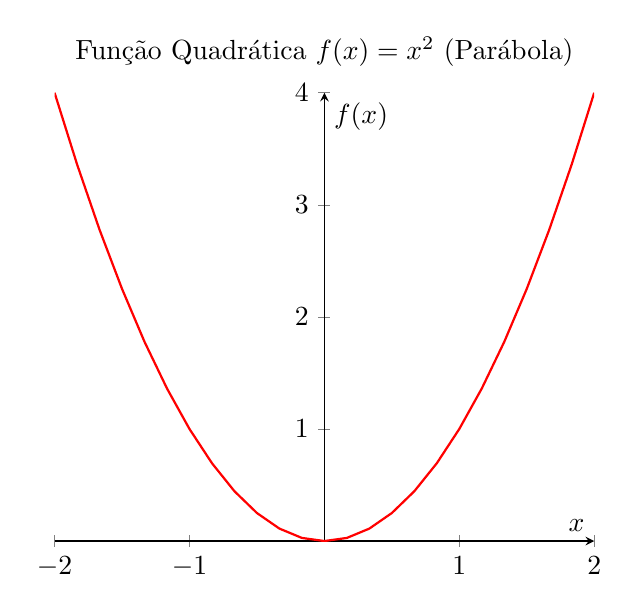
\begin{tikzpicture}
    \begin{axis}[
        title={Função Quadrática $f(x)=x^2$ (Parábola)},
        axis lines=middle,
        xlabel={$x$},
        ylabel={$f(x)$},
        xmin=-2, xmax=2, ymin=0, ymax=4]
    \addplot[red, thick, domain=-2:2] {x^2};
    \end{axis}
    \end{tikzpicture}
    \caption{Gráfico de uma função quadrática $f(x)=x^2$, representando uma parábola.}
    \label{fig:funcao_quadratica}
\end{figure}

% -----------------------------------------------
% ---------------3. FUNÇÃO SENOIDE--------------- 
% -----------------------------------------------
\begin{figure}[H]
    \centering
    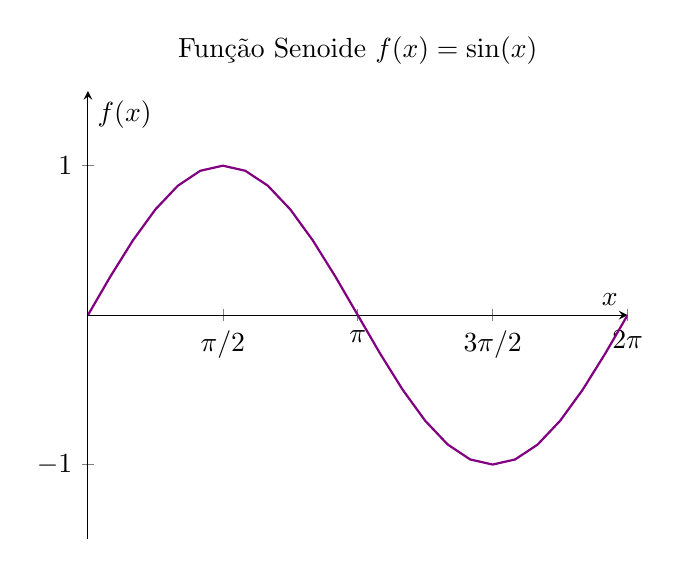
\begin{tikzpicture}
    \begin{axis}[
        title={Função Senoide $f(x)=\sin(x)$},
        axis lines=middle,
        xlabel={$x$},
        ylabel={$f(x)$},
        xmin=0, xmax=360, ymin=-1.5, ymax=1.5,
        xtick={0, 90, 180, 270, 360},
        xticklabels={0, $\pi/2$, $\pi$, $3\pi/2$, $2\pi$}
    ]
    \addplot[violet, thick, domain=0:360] ({x}, {sin(x)});
    \end{axis}
    \end{tikzpicture}
    \caption{Gráfico da função senoide $f(x)=\sin(x)$, demonstrando periodicidade.}
    \label{fig:funcao_senoide}
\end{figure}

% -----------------------------------------------
% -------------4. FUNÇÃO EXPONENCIAL------------- 
% -----------------------------------------------
\begin{figure}[H]
    \centering
    \begin{tikzpicture}
    \begin{axis}[
        title={Função Exponencial $f(x)=e^x$},
        axis lines=middle,
        xlabel={$x$},
        ylabel={$f(x)$},
        xmin=-2, xmax=2, ymin=0, ymax=8,
        domain=-2:2]
    \addplot[green!60!black, thick] {exp(x)};
    \end{axis}
    \end{tikzpicture}
    \caption{Gráfico de uma função exponencial $f(x)=e^x$, representando crescimento acentuado.}
    \label{fig:funcao_exponencial}
\end{figure}

% -----------------------------------------------
% -------------5. FUNÇÃO LOGARÍTMICA------------- 
% -----------------------------------------------
\begin{figure}[H]
    \centering
    \begin{tikzpicture}
    \begin{axis}[
        title={Função Logarítmica $f(x)=\ln(x)$},
        axis lines=middle,
        xlabel={$x$},
        ylabel={$f(x)$},
        xmin=0, xmax=5, ymin=-2, ymax=2,
        domain=0.01:5]
    \addplot[orange, thick] {ln(x)};
    \end{axis}
    \end{tikzpicture}
    \caption{Gráfico da função logarítmica natural $f(x)=\ln(x)$, mostrando o crescimento lento.}
    \label{fig:funcao_logaritmica}
\end{figure}
% -----------------------------------------------


\newpage % Nova Página 
% -----------------------------------------------
\section{Exemplo de Lista de Tabelas}
% -----------------------------------------------

\noindent Esta seção demonstra a correta formatação ABNT para tabelas e garante o preenchimento da Lista de Tabelas.

% -----------------------------------------------
\begin{table}[H]
    \centering
    \caption{Resultados dos Testes de Velocidade (Baseline)}
    \label{tab:velocidade_baseline}
    \begin{tabular}{lcc}
        \toprule
        Módulo & Tempo (ms) & Status \\
        \midrule
        Login & 120 & OK \\
        Busca & 450 & Crítico \\
        \bottomrule
    \end{tabular}
\end{table}

\begin{table}[H]
    \centering
    \caption{Recursos Utilizados por Componente}
    \label{tab:recursos_comp}
    \begin{tabular}{lrr}
        \toprule
        Componente & RAM (MB) & CPU (\%) \\
        \midrule
        Backend API & 512 & 30 \\
        Frontend UI & 128 & 15 \\
        \bottomrule
    \end{tabular}
\end{table}

\begin{table}[H]
    \centering
    \caption{Cronograma de Implementação (Fase Alpha)}
    \label{tab:cronograma_alpha}
    \begin{tabular}{llr}
        \toprule
        Tarefa & Responsável & Prazo (Dias) \\
        \midrule
        Setup Inicial & Equipe T.I. & 5 \\
        Desenvolvimento & Programador & 15 \\
        \bottomrule
    \end{tabular}
\end{table}

\begin{table}[H]
    \centering
    \caption{Classificação de Bugs por Prioridade}
    \label{tab:bugs_prioridade}
    \begin{tabular}{lc}
        \toprule
        Prioridade & Incidência \\
        \midrule
        Crítica & 3 \\
        Média & 8 \\
        Baixa & 12 \\
        \bottomrule
    \end{tabular}
\end{table}

\begin{table}[H]
    \centering
    \caption{Comparativo de Linguagens de Programação}
    \label{tab:linguagens_comp}
    \begin{tabular}{ccc}
        \toprule
        Linguagem & Desempenho & Curva de Aprendizado \\
        \midrule
        Python & Médio & Baixa \\
        C++ & Alta & Alta \\
        \bottomrule
    \end{tabular}
\end{table}

\begin{table}[H]
    \centering
    \caption{Especificações do Painel Fotovoltaico}
    \label{tab:painel_foto}
    \begin{tabular}{lc}
        \toprule
        Parâmetro & Valor \\
        \midrule
        Potência Máx. & 350 W \\
        Eficiência & 20.5\% \\
        \bottomrule
    \end{tabular}
\end{table}
% -----------------------------------------------


% -----------------------------------------------
% -------------PARTE - Resultados---------------
% -----------------------------------------------
\part{Resultados}

\chapter{Suspendisse vel felis}

\section{Praesent enim elit}
\lipsum[6-7] % Gera texto de exemplo para preencher a página. 

\section{Curabitur et nunc}
\lipsum[8-10] % Gera texto de exemplo para preencher a página. 


% ----------------------------------------------------------
% Finaliza a parte no bookmark do PDF
% para que se inicie o bookmark na raiz
% e adiciona espaço de parte no Sumário
% ----------------------------------------------------------
\phantompart


% -----------------------------------------------
% ----------------Conclusão----------------------
% -----------------------------------------------
\chapter{Conclusão}
% -----------------------------------------------
\lipsum[31-33] % Gera texto de exemplo para preencher a página.


% -----------------------------------------------
% -----------ELEMENTOS PÓS-TEXTUAIS--------------
% -----------------------------------------------
\postextual


% -----------------------------------------------
% ----------Referências bibliográficas-----------
% -----------------------------------------------
\chapter*{Referências}                                               % Insere o título
\markboth{Referências}{Referências}                                  % Título "Referências" no cabeçalho.
\addtocontents{toc}{\protect\vspace{\baselineskip}}                  % Adiciona uma linha.
\addcontentsline{toc}{chapter}{\protect\MakeUppercase{REFERÊNCIAS}}  % Nível 'chapter' para linha grossos.
\printbibliography[heading=none]                                     % Imprime a bibliografia.
% -----------------------------------------------



% -----------------------------------------------
% -----------------APÊNDICE---------------------- 
% -----------------------------------------------
\begin{apendicesenv}
\partapendices % Imprime uma página indicando o início dos apêndices

\chapter{Quisque libero justo}

\section{Aliquam viverra arcu}
\lipsum[8-9] % Gera texto de exemplo para preencher a página. 

\section{Mauris consequat}
\lipsum[24] % Gera texto de exemplo para preencher a página. 

% -----------------------------------------------

\chapter{Nullam elementum}

\section{Quisque facilisis auctor sapien}
\lipsum[80-81] % Gera texto de exemplo para preencher a página. 

\section{Aliquam quis quam non metus}
\lipsum[34] % Gera texto de exemplo para preencher a página. 

\end{apendicesenv}
% -----------------------------------------------


% -----------------------------------------------
% ------------------ANEXOS-----------------------
% -----------------------------------------------
\begin{anexosenv}
\partanexos % Imprime uma página indicando o início dos anexos

\chapter{Morbi ultrices rutrum lorem}

\section{Pellentesque sodales}
\lipsum[40-41] % Gera texto de exemplo para preencher a página. 

\section{Curabitur diam tortor}
\lipsum[54-55] % Gera texto de exemplo para preencher a página. 

\end{anexosenv}
% -----------------------------------------------

\end{document} 